% Template for a Computer Science Tripos Part II project dissertation
\documentclass[12pt,a4paper,twoside,openright]{report}
\usepackage[pdfborder={0 0 0}]{hyperref}    % turns references into hyperlinks
\usepackage[margin=25mm]{geometry}  % adjusts page layout
\usepackage{graphicx}  % allows inclusion of PDF, PNG and JPG images
\usepackage{verbatim}
\usepackage{docmute}   % only needed to allow inclusion of proposal.tex
\usepackage{fancyvrb}
\usepackage{color}
\usepackage{amsmath}
\usepackage{subcaption}


\DefineVerbatimEnvironment{blockcode}
  {Verbatim}
  {fontsize=\small}

\raggedbottom                           % try to avoid widows and orphans
\sloppy
\clubpenalty1000%
\widowpenalty1000%

\renewcommand{\baselinestretch}{1.1}    % adjust line spacing to make
                                        % more readable

\begin{document}

\bibliographystyle{plain}


%%%%%%%%%%%%%%%%%%%%%%%%%%%%%%%%%%%%%%%%%%%%%%%%%%%%%%%%%%%%%%%%%%%%%%%%
% Title


\pagestyle{empty}

\rightline{\LARGE \textbf{George Ash}}

\vspace*{60mm}
\begin{center}
\Huge
\textbf{} \\[5mm]
Computer Science Tripos -- Part II \\[5mm]
Fitzwilliam College \\[5mm]
\today  % today's date
\end{center}

%%%%%%%%%%%%%%%%%%%%%%%%%%%%%%%%%%%%%%%%%%%%%%%%%%%%%%%%%%%%%%%%%%%%%%%%%%%%%%
% Proforma, table of contents and list of figures

\pagestyle{plain}

\chapter*{Proforma}

{\large
\begin{tabular}{ll}
Name:               & \bf George Ash                       \\
College:            & \bf Fitzwilliam College                     \\
Project Title:      & \bf Smart Antialiasing for Virtual Reality \\
Examination:        & \bf Computer Science Tripos -- Part II, July 2017  \\
Word Count:         & \bf 1587\footnotemark[1] \\
Supervisor:         & Dr Rafal Mantiuk                    \\ 
\end{tabular}
}
\footnotetext[1]{This word count was computed
by \texttt{detex diss.tex | tr -cd '0-9A-Za-z $\tt\backslash$n' | wc -w}
}
\stepcounter{footnote}


\section*{Original Aims of the Project}

To examine the effect on the image quality and GPU load when applying antialiasing only to a small field of view in a consumer Virtual Reality (VR) Headmounted Display (HMD).


\section*{Work Completed}

Implementation of a generic, method to antialiase only in the centre of the screen using OpenGL. Examined an implementation to accomodate to Foveated Rendering and multi-resolution rendering.
A user study was conducted that determined image quality across a range of antialiasing techniques.

\section*{Special Difficulties}

Learning to profile accurately GPU software.
Learning OpenGL in depth.
 
\newpage
\section*{Declaration}

I, [Name] of [College], being a candidate for Part II of the Computer
Science Tripos [or the Diploma in Computer Science], hereby declare
that this dissertation and the work described in it are my own work,
unaided except as may be specified below, and that the dissertation
does not contain material that has already been used to any substantial
extent for a comparable purpose.

\bigskip
\leftline{Signed [signature]}

\medskip
\leftline{Date [date]}

\tableofcontents

\listoffigures

\newpage
\section*{Acknowledgements}

This document owes much to an earlier version written by Simon Moore
\cite{Moore95}.  His help, encouragement and advice was greatly 
appreciated.

%%%%%%%%%%%%%%%%%%%%%%%%%%%%%%%%%%%%%%%%%%%%%%%%%%%%%%%%%%%%%%%%%%%%%%%
% now for the chapters

\pagestyle{headings}

\chapter{Introduction}

\section{Background}

Through the affordability of display panels and cheap wide-angle lenses, Virtual Reality Displays are beggining to flood the consumer market. To meet this demand, efficient rendering software and practices will need to be adopted.

Graphics rendering pipelines take good advantage of available GPU power. But the constraints of realistic, immersive virtual reality present a huge challenge to engineers. They must output a high resolution, wide field of view, antialiased image, with a response to stimulus time under 20ms.

As this technology progresses and matures, it will become increasingly important to provide low-latency response times. Resolutions will need to increase to around 8K*8K, but to achieve this our graphics processing hardware and software will have to evolve too.

Aliasing in graphics refers to spatial and temporal artefacts present in a rendered image. They are the result of sampling a higher frequency signal component at a lower freqency.

Antialising is the process of removing such artefacts, but this has to be done efficiently or we will sacrifice frame drops and potential motion sickness for the end-user.
There are a multitude of antialiasing approaches, though most sample at a higher frequency than will be presented in the final image, then downsampling through some filter. 

\section{Common Antialiasing Approaches}

There are a multitude of antialising approaches, one of the most common is Supersampled Anti-alising (SSAA).
First the scene is sampled at an integer multiple higher resolution than we intend to present it.
Then, before presenting, this image is downsampled by taking for each pixel in the presented image, a linear combination of its closest neighbors in the higher resolution image. In the figure below, to calculate the final pixels colour, 4 samples per pixel are computed, each run through some downsampling filter, each providing a quarter of the color for the final, presented image. The formula for for determining the final colour of the pixel is the simple mean average for each colour (Red, Green and Blue):
$$ c = \frac{1}{n}\displaystyle\sum_{i=1}^n c_i $$ where n is the number of samples per pixels we take.



\begin{figure}
\setlength{\unitlength}{1mm}-
\begin{center}
\begin{picture}(125,100)

\put(10,65){High-res image}

\put(0,40){\framebox(20,20){$1_1$}}
\put(20,40){\framebox(20,20){$1_2$}}
\put(0,20){\framebox(20,20){$1_3$}}
\put(20,20){\framebox(20,20){$1_4$}}

\put(40,55){\vector(1,0){20}}
\put(40,45){\vector(1,0){20}}
\put(40,25){\vector(1,0){20}}
\put(40,35){\vector(1,0){20}}

\put(50,75){Subsample Resolve}
\put(60,10){\framebox(10,60)}

\put(70,33){\vector(1,0){20}}
\put(70,38){\vector(1,0){20}}
\put(70,43){\vector(1,0){20}}
\put(70,48){\vector(1,0){20}}

\put(88,55){Presented Image}
\put(90,30){\framebox(20,20){1}}



\end{picture}
\end{center}
\caption{An example of 4x Supersampling for a single pixel.}
\label{latexpic1}
\end{figure}

Another common approach, that is built into the OpenGL API, is Multisampled Anti-aliasing (MSAA). As before, the scene is sampled at a higher resolution than we intend to present it, forming a coverage mask for each pixel. If any of the samples in this coverage mask are covered by a triangle, we need to run a fragment shader for this pixel. The result of the fragment shader is applied to all relevant subsamples in the coverage mask. We therefore don't have to run a fragment shader for every subsample in the pixel, only those that are covered by multiple triangles.
MSAA provides a significant speedup over SSAA and is widely employed in practice, but only removes spatial artefacts at polygon edges. SSAA can remove artefacts within polygons, an example of which will be presented later.

\section{Virtual Reality Headmounted Displays}

A typical virtual Reality Headmounted Display (HMD) is comprised of 2 main components: The screen - to which our rendered image is presented and a wide-angle lens - to project the displayed image into the eye. The lens allows for the user to focus on a screen that is normally too close for the eye to focus on by itself. 
Side effects of the lens used in the Oculus Rift DK2 are chromatic abberation, pincushion distortion, and astigmatism.\\

Chromatic abberation refers to the separation of colour due to the different refractive indexes for different wavelengths of light. A Virtual Reality API should correct for this.\\

Pincushion distortion refers to the stretching of the image near the egdes. The inverse of pincushion distortion, barrel disortion, can be applied to reverse the effects of pincushion distortion. The barrel distortion that the Oculus SDK applies results in a varying number of texels per pixel in our final image, a property will be explored in the second extension.


\begin{figure}[tbh]
\centerline{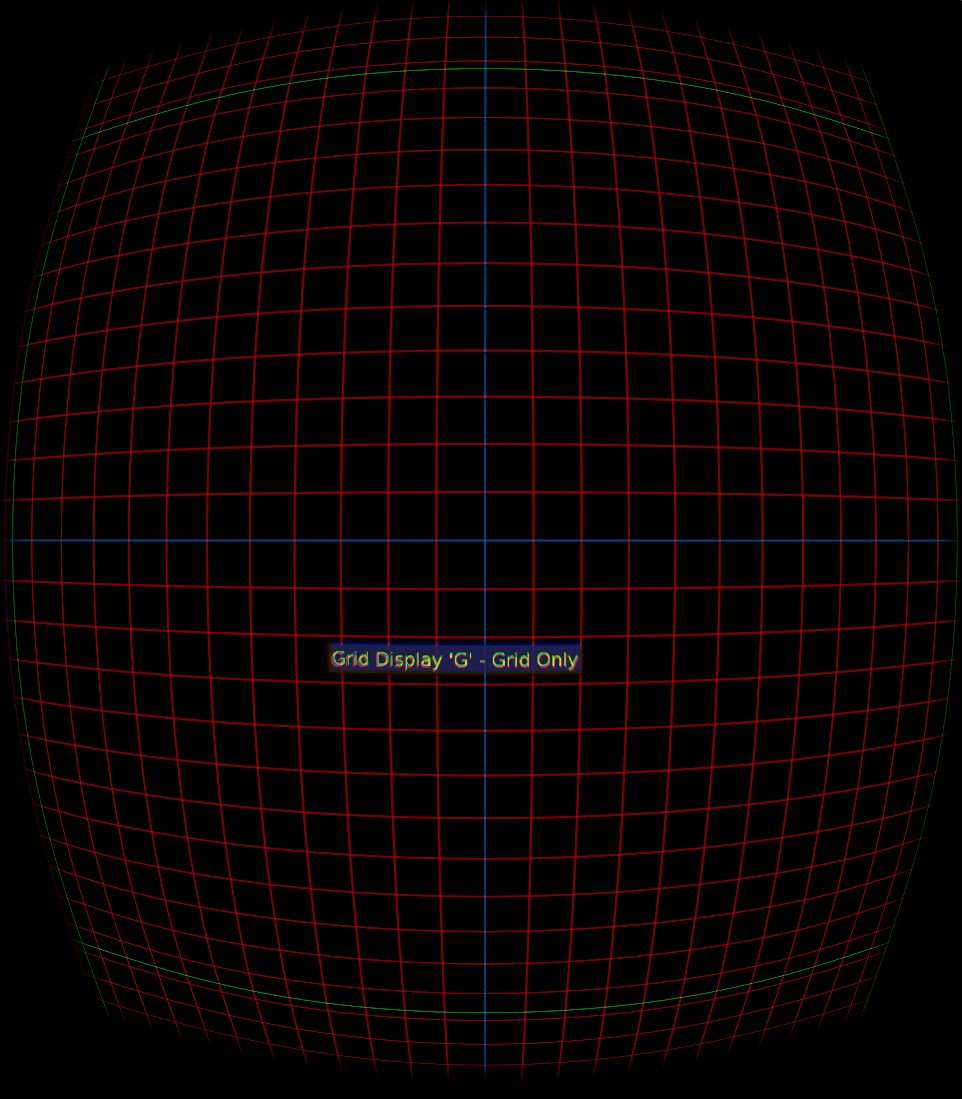
\includegraphics[width=10cm]{figs/distortiongrid.png}}
\caption{Barrel distortion applied to a rectangular grid}
\label{distortiongrid}
\end{figure}

Lens astigmatism is a property of the lenses used in most consumer HMDs. Because of the astigmatism, the image presented to the user is sharp in the center but becomes progressivelly blurrier as you look towards the edges.  It can be corrected for by adding more lenses to the HMD, but this ends up being too expensive and bulky for consumer versions.

\begin{figure}
\centerline{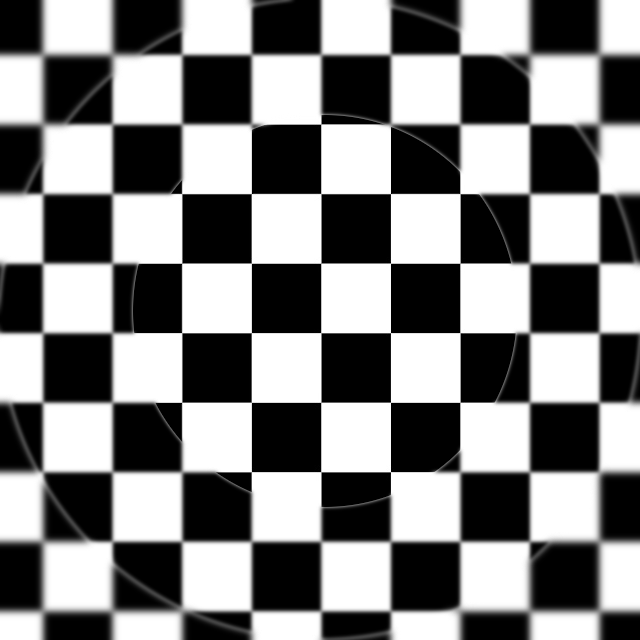
\includegraphics[width=6cm]{figs/blur.png}}
\caption{A depiction of lens astigmatism. The percieved image blurs as you move away from the sharp center.}
\label{blurred}
\end{figure}

This property can be exploited by antialiasing only where the image is sharpest, in the center. Graphical artefacts at the edges should be blurred enough to be unnoticable. It is this principle that we'll develop the following antialiasing approaches on top of.

\chapter{Preparation}

This chapter outlines any preparatory work that was done before implementation of the two antialiasing approaches.

\section{OpenGL}

The OpenGL API provides an interface to render 3D graphics. It's cross language, with native C/C++ bindings, well documented, and the most widely adopted open source graphics API. As a bonus it supports some efficient antialising standards.

Below I describe some OpenGL terminology that will be used lots later.

\begin{description}

\item\texttt{Framebuffer} \\
  A collection of buffers that can be used as the destination for rendering.

\item\texttt{Blitting} \\
  The process of moving image data between framebuffers.

\item\texttt{Front Buffer} \\
  The buffer containing the image that is presented onscreen now. This buffer is contained within the Default Framebuffer.

\item\texttt{Back Buffer} \\
  The buffer containing the image that will be presented onscreen in the next frame, is contained within the Default Framebuffer. 

\item\texttt{Primitive} \\
  An interpretive scheme used to determine what a stream of vertices represents when being rendered. For example \texttt{GL\_POINTS} causes each vertex to be interpreted as a point. Other primitive types include \texttt{GL\_TRIANGLES} amd \texttt{GL\_LINES}
\item\texttt{Fragment} \\
  Collection of values produced by the rasterizer. A fragment represents a sample-sized segment of a rasterized primitive. These are processed by the fragment shader. 
\end{description}

\subsection{The OpenGL pipeline}

OpenGL provides a pipeline through which data about the rendered scene is processed and rasterized. A simplified view of it is presented here, given that some stages are optional or non-programmable.


\begin{figure}
\setlength{\unitlength}{0.8mm}-
\begin{center}
\begin{picture}(80,120)

\put(0,100){\framebox(80,10){Vertex Data}}
\put(0,80){\framebox(80,10){Vertex Shader}}
\put(0,60){\framebox(80,10){Geometry Shader}}
\put(0,40){\framebox(80,10){Primitive Assembly, Rasterization}}
\put(0,20){\framebox(80,10){Fragment Shader}}
\put(0,0){\framebox(80,10){Per Sample Operations}}



\put(40,20){\vector(0,-1){10}}
\put(40,40){\vector(0,-1){10}}
\put(40,60){\vector(0,-1){10}}
\put(40,80){\vector(0,-1){10}}
\put(40,100){\vector(0,-1){10}}




\end{picture}
\end{center}
\caption{A glimpse at the OpenGL rendering pipeline}
\label{latexpic2}
\end{figure}

Vertex data enters the pipeline, typically it has been uploaded to the GPU through a \texttt{Vertex Buffer Object}. Each vertex usually has associated data such as a colour, a normal vector, and texture coordinates.\\
The Vertex Shader is run for every vertex in the scene. In the typical case it transforms vertexes in 3d world space to window space coordinates. Vertex data from the previous scene is bound in through named variables.\\

The Geometry Shader is run for every primitive in the scene (in all of the implementations here I've simplified these to triangles as a general case). It is an unusual stage in that it can amplify geometry, outputting more primitives than it takes as input. This stage is optional, but it's used later on.\\

The Fragment shader is run for every fragment in the window space, it is typically used to perform lighting and texturing for the scene.

\section{Development}

Being relatively new to OpenGL I decided to build a toy renderer to teach myself the basics of the API.

This toy renderer proved invaluable to the success of the project, since I knew and understood the source code completely, I could implement and test an idea for optimisation or an implementation strategy quickly. The toy renderer was implemented in C++.

To get an idea of how these implementations would fare in a larger, more computationally intensive renderer I decided to modify the demo provided with the Oculus SDK 5.0.1: OculusWorldDemo.
The codebase to this was in C++ and the rendering code was written to be extensible - allowing for different graphics APIs to implement lower level rendering calls. The OpenGL implementation was Open Source and under the Apache License.

An agile approach was taken when implementing the antialising methods, stories were broken up into small, managable chunks. After these were implemented - extensions could be written up and implemented on top.
Unit tests were written for all new methods. However, where methods and classes were extended beyond Oculus' implementation, unit tests were not added due to the high degree of coupling within OculusWorldDemo and OpenGL and the extensive API mocking required. To make up for this, and to ensure correctness, runtime assertions were made on all branches and method calls.

\section{Software libraries}

The OculusVR SDK was used in the Demo to interface with the Oculus Rift DK2 HMD. An outdated version 0.5.0.1 was used being the last version to support linux.
The SDK provided vector and matrix math modules, runtime assertions, and allowed barrel distortion and chromatic abberation to be performed.

GLFW was used for context creation in the toy renderer.
GLM was used for matrix math in the toy renderer.

\section{Programming Languages}

C++ was used in both the toy renderer and OculusWorldDemo. It has native OpenGL bindings and has extensive compiler support allowing for performance to be maximised.

GLSL is the OpenGL C-like shader language that is run on the GPU. It was used to implement the first and second extensions. It's syntax is very similar to C. Learning it was not particularly time-consuming.

\section{Development Tools}

\begin{itemize}
\item Sublime text was the editor used to write all the software here.

\item The C/C++ debugger \texttt{gdb} was used to debug both the toy renderer and OculusWorldDemo.

\item AMD's GPUPerfStudio was used to profile both OculusWorldDemo and the toy renderer.

\item \texttt{BuGLe} was used to debug the OpenGL calls in both the toy renderer and OculusWorldDemo.

\end{itemize}
\subsection{Version Control}

Git was used as a version control system due to its flexibility and my familiarity with it. Remote repositories were placed both on a separate harddrive and Github. These remotes were updated on every commit. Commits were made after every development story was completed.

\subsection{Failsafes}

In the event of failure of my development machine, MCS machines were compatible and tested with the software I was using. Also two backups were made of all changes to the codebase, detailed above.

\chapter{Implementation}

\section{OculusWorldDemo Structure}

Given that the implementation of two antialiasing techniques is built on top of Oculus' existing work, it was first neccesary to understand a large portion of their codebase.
Here I give a brief overview of system components that will be modified and used later on. I also give a brief overview of Oculus' SDK before detailing components that were added and modified to OculusWorldDemo.

\begin{itemize}
\item OculusWorldDemoApp \\
  The class describing the application OculusWorldDemo, contains high level rendering instructions, calculcation of HMD values, user input (Mouse, Keyboard), state initilisation and more.

\item RenderDevice \\
  The module containing rendering state and methods, called by OculusWorldDemoApp. Provides several implentations of its methods in DirextX and OpenGL. Handles shader compilation, linking, GPU memory allocation for vertex \& texture data and more.

\end{itemize}
\section{The Render Loop}
At every frame, the Oculus SDK provides headtracking information that must be used to maintain the appropriate user position and orientation in the program.

The bulk of rendering code is done within the OculusWorldDemoApp::OnIdle() method, which determines if and when a frame should be drawn, along with other bookeeping.
For each frame the following must be done:

\begin{itemize}
  \item The SDK call \texttt{ovrHmd\_BeginFrame()} should be called to mark the beginning of the frame.
  \item Update headtracking state.
  \item Draw the scene to some texture(s) $\tau$.
  \item Call \texttt{ovrHmd\_EndFrame($\tau$)}.
\end{itemize}

The Oculus SDK then takes $\tau$ and applies barrel distortion and chromatic abberation through a post-processing stage. 

\section{Barrel Distortion}

A common model used to model barrel distortion is Brown's distortion model. 

\[
f(\vec p) = \frac{\vec(p)}{1-\alpha\vec(p)}
\]
Where $\vec(p)$ is some point in the source image, and $\alpha$ is the amount of disortion applied to the image, and is a property of the lens.


\begin{figure}[tbh]
\begin{center}
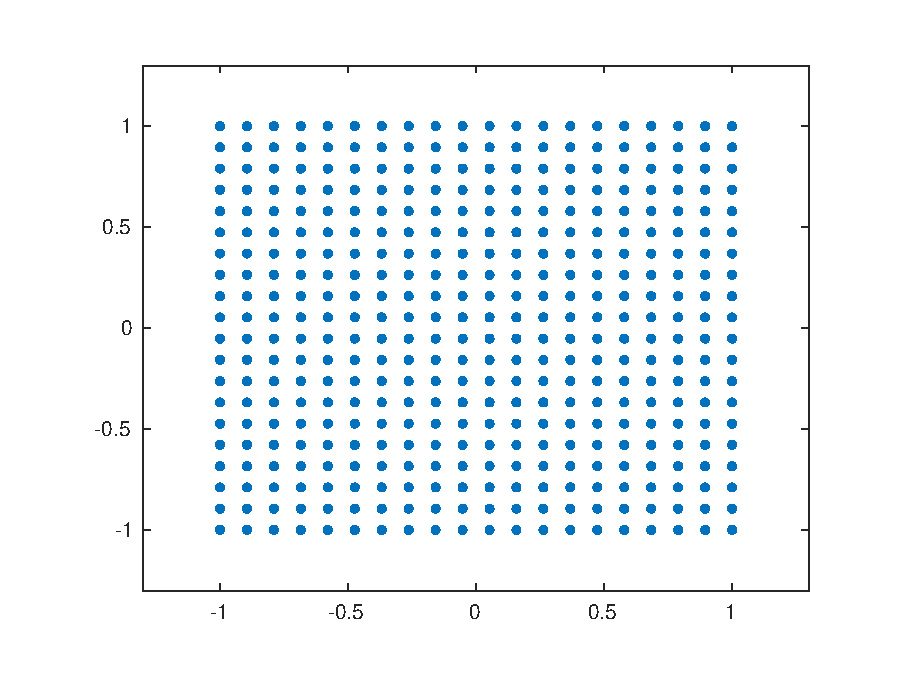
\includegraphics[width=6cm]{figs/pre_distortion.eps}
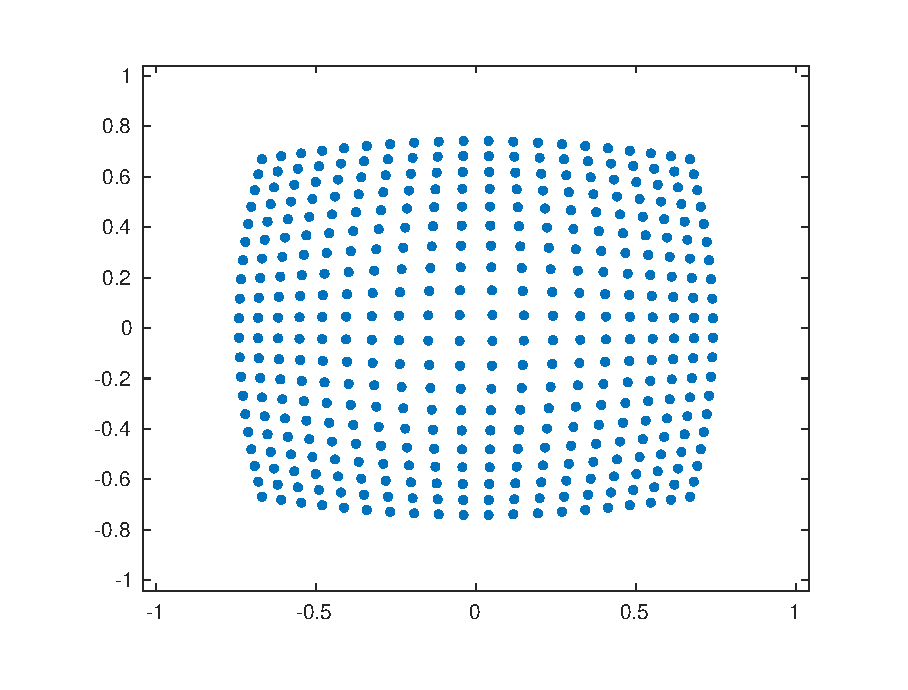
\includegraphics[width=6cm]{figs/post_distortion.eps}
\caption{Shows a regular pixel grid pre and post brown distortion. Coordinates are normalised to the range $[-1,1]$}
\label{epsfig1}
\end{center}
\end{figure}

The method used implement barrel distortion in a graphics API has evolved over the past few years. Initially, the distortion was calculated as a post-processing step in the fragment shader. Later, the image provided to the post-processing step was used to texture a mesh that had distortion applied to it. The latter approach is adopted by the Oculus SDK 5.0.1. Another approach can be built into the rendering pipeline in the vertex shader, it removes the need for post-processing, but additionally requires the use of tesselation.

\section{Implementation overview} 

To achieve antialiasing in the centre of the image using OpenGL we are required to draw the scene twice for each eye. Once for the antialiased, low field of view centre, and one for the lower quality border. To implement this we are required to set up render targets for each field of view, along with projection matrices for each, and finally some method to blend the two render targets together before presenting the final frame.

\section{Projection Transformation}

An essential component to 3D graphics is the projection transformation. It takes as input 3D coordinates and maps them to 2D window coordinates.
Two types of projection must be dealt with in the implementation. 

\subsection{Orthographic projection}
The orthographic projection is a form of parralel projection, where all projection lines are parralel to the \texttt{lookAt} vector /*TODO*/ define. 

\[
\begin{pmatrix}
\dfrac{2}{right-left} & 0 & 0 & -\dfrac{right+left}{right-left} \\
0 & \dfrac{2}{top-bottom} & 0 & -\dfrac{top+bottom}{right-left} \\
0 & 0 & \dfrac{2}{far-near} & -\dfrac{far + near}{far-near} \\
0 & 0 & 0 & 1
\end{pmatrix}
\]

This matrix is used to render two dimensional information at a required distance from the user. In OculusWorldDemo and others it is used to render UI components.
\subsection{Perspective projection}

The perspective projection is also used to render 3D scenes.
\[
\begin{pmatrix}
\dfrac{2*near}{right-left} & 0 & \dfrac{right + left}{right - left} & 0 \\
0 & \dfrac{2*near}{top-bottom} & \dfrac{top+bottom}{top-bottom} & 0 \\
0 & 0 & -\dfrac{far + near}{far-near} & -\dfrac{-2far*near}{far-near} \\
0 & 0 & -1 & 0
\end{pmatrix}
\]

To project onto a smaller portion of the screen we have to specify alternate orthographic and perspective projection matrices that correspond to the smaller viewing frustrum in the center of the screen. In OculusWorldDemo we can specify new matrices: \texttt{OrthoProjectionSmall} and \texttt{OrthoProjection}. 

\subsection{Matrix Initilisation}

The Oculus SDK will provide to the programmer the estimated field of view from the vector going from the eye to the center of the image. This information can be used to construct a frustum and projection matrix use in rendering.

\begin{figure}[tbh]
\centerline{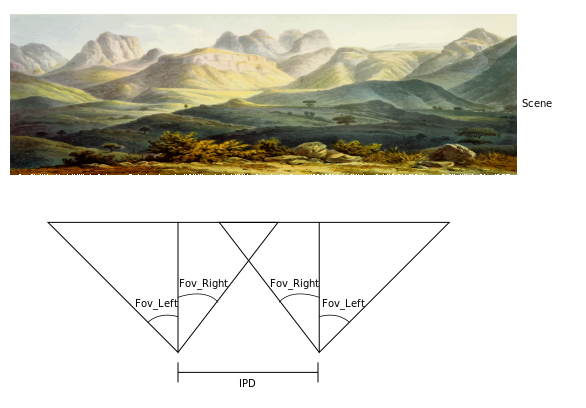
\includegraphics[scale=0.6]{figs/asymmetrical_fov.png}}
\caption{Shows the field of view for each eye. Not shown are the fov\_Up and fov\_Down parameters}
\label{epsfig1}
\end{figure}

This information can be used to compute a matrix for both the full field of view and reduced, central field of view.

In the common case however, given a matrix \texttt{m} representing the projection for a full, symmetric field of view, the matrix for a smaller field of view can be computed with the following method.

\begin{blockcode}
Matrix4f centeredSmallMatrix(Matrix4f m, float ratio){
    Matrix4f rtn; 
    rtn = copyMatrix(m);
    rtn.M[0][0] *= ratio; //vertical FOV * 1/ratio
    rtn.M[1][1] *= ratio; //horizontal FOV * 1/ratio
    return rtn;
}
\end{blockcode}

The above returns a projection matrix whose near planes dimensions are $\frac{1}{\texttt{ratio}}$ of the input projection matrix's near plane. Figure XXXX illustrates this. This small matrix will correspond to the smaller field of view whose render target will have higher quality antialiasing applied. 

/*TODO*/ insert split fov image here. 

\section{Allocating Textures}

The framebuffer we render to must be complete before we begin rendering to it, so textures must be allocated and formatted properly beforehand. This section will describe texture allocation in OpenGL, and how the implementation in OculusWorldDemo was modified to permit the approach outlined before. 
 
The Oculus SDK provides a method \texttt{ovrHmd\_GetFovTextureSize()} that returns a reccomended texture size for a given Field of View and pixel density at the centre of the screen.

The code below outlines the process for allocating a framebuffer in OpenGL that contain render target textures that are $frac{1}{r}$ the size of the destination texture.

\begin{blockcode}

\end{blockcode}
/*TODO*/ define and explain


\section{Drawing the scene}

The perspective transformation is usually performed in the vertex shader stage, so the perspective transformation matrix must be linked up to this stage.

\begin{blockcode}
/*TODO*/ vertex shader code
\end{blockcode} 
This matrix can be linked up to the vertex shader with the function \texttt{glUniformMatrix4fv()}.

The render method of each scene needs only to know which eye it is rendering to, and whether it is drawing to the center or the borders of the image. 
So the render method in OculusWorldDemoApp was modified to include the perspective projection matrix of the portion of the scene it is drawing to.

\begin{blockcode}[commandchars=\\\{\}]
void OculusWorldDemoApp::RenderEyeView(ovrEyeType eye,
                                       \color{green}Matrix4f * projection,
                                       \color{green}Matrix4f * orthoProj)
\end{blockcode}

We can then bind the correct projection matrices inside this method with a call to \texttt{glUniformMatrix4fv()}
Nothing else needs altering in the draw call for this implementation.

\subsection{Modifying The Render Loop}

Before we can begin rendering to each view with corresponding framebuffer $F$, OpenGL state needs to be set up. Therefore for each framebuffer $F$ we need to perform the following inside of the render loop. 4 Framebuffers can be used to achieve a stereoscopic view with subscreen multisampling or supersampling.

\begin{enumerate}

\item Bind $F$ to the draw framebuffer.
\item Set the viewport to the resolution of $F$.
\item Draw the scene onto $F$.

\end{enumerate}

As I will describe later on, this process can be handled on the GPU side with the use of the geometry shader, freeing up the CPU and reducing the number of draw calls to a half (or a quarter if stereoscopic rendering is used).

\section{MultiSample Resolve}

With a multisampled or supersampled texture along with a single sampled border texture, a resolve from the multisampled or supersampled texture to the destination buffer needs to be performed to merge the two together before presenting onscreen. This can be achieved with a blit operation or blending in a post-processing stage.
The function below takes as arguments a multisampled or supersampled texture along with an output texture. It then resolves the samples from the source texture to the target texture. The method doesn't care whether the source texture is multisampled or supersampled, these cases will be identified from the source texture's flags.

\begin{blockcode}[commandchars=\\\{\}, numbers=left]
void RenderDevice::ResolveMsaa(OVR::Render::Texture* msaaTex, OVR::Render::Texture* outputTex, float ratio)
\{
    bool isMsaaTarget = msaaTex->GetSamples() > 1;
    glBindFramebuffer( GL_READ_FRAMEBUFFER, MsaaFbo);
    glFramebufferTexture2D( GL_READ_FRAMEBUFFER, GL_COLOR_ATTACHMENT0,
                            isMsaaTarget ? GL_TEXTURE_2D_MULTISAMPLE : GL_TEXTURE_2D,
                            ((Texture*)msaaTex)->TexId, 0);
    glFramebufferRenderbuffer(GL_READ_FRAMEBUFFER, GL_DEPTH_ATTACHMENT, GL_RENDERBUFFER, 0);
    OVR_ASSERT(glCheckFramebufferStatus(GL_READ_FRAMEBUFFER) == GL_FRAMEBUFFER_COMPLETE);

    glBindFramebuffer( GL_DRAW_FRAMEBUFFER, CurrentFbo );
    glFramebufferTexture2D(GL_DRAW_FRAMEBUFFER, GL_COLOR_ATTACHMENT0, GL_TEXTURE_2D, ((Texture*)outputTex)->TexId, 0);
    glFramebufferRenderbuffer(GL_DRAW_FRAMEBUFFER, GL_DEPTH_ATTACHMENT, GL_RENDERBUFFER, 0);

    OVR_ASSERT(glCheckFramebufferStatus(GL_DRAW_FRAMEBUFFER) == GL_FRAMEBUFFER_COMPLETE);

\color{green}    int off_x = (outputTex->GetWidth() - outputTex->GetWidth()/ratio)/2; //Offset from bottom left of the target texture we wish to blit the source to. 
\color{green}    int off_y = (outputTex->GetHeight() - outputTex->GetHeight()/ratio)/2; // ditto
\color{green}    glBlitFramebuffer( 0, 0, msaaTex->GetWidth(), msaaTex->GetHeight(), off_x, off_y,
\color{green}                             off_x + outputTex->GetWidth()/ ratio,
\color{green}                             off_y + outputTex->GetHeight()/ ratio,
\color{green}                             GL_COLOR_BUFFER_BIT, GL_LINEAR);

    glBindFramebuffer( GL_FRAMEBUFFER, 0 );  
    GLint err = glGetError();
    OVR_ASSERT_AND_UNUSED(!err, err);
\}
\end{blockcode}

The method needs to set up the OpenGL state machine for the \texttt{glBlitFramebuffer} on line 21. First a multisampled framebuffer is set up to be read in line 2. Next we associate this framebuffer with \texttt{msaaTex} in lines 3-4. 
We then set up the destination texture in its own framebuffer, and set the GL state to draw to this buffer in the blit in lines 11-13.

Note that assertions are made to check for framebuffer completeness. An imcomplete framebuffer cannot be drawn to.

Lines 19-24 implement the last stage of the downsampling method given in Y. We only blit the color buffer and do a linear downsample. 

The GL\_LINEAR filter will perform a supersample resolve by taking a weighted linear combination of the destination texels nearest neighbors in the source texture. Given that the source textures texels are equally spaced, this linear filter implements the average given in section BALRA.

If the input texture is multisampled, and if the source and destination rectangles are the same size, OpenGL will perform a multisample resolve onto the destination framebuffer in hardware.

\section{OpenGL optimisations}

As a summary of the implementation so far, each frame has to be rendered in the following way:

\begin{itemize}
  \item Set the viewport and projection matrix for the inner field of view.
  \item Render a multisampled or supersampled view of the scene onto some render target.
  \item Set the viewport and projection matrix for the outer field of view.
  \item Render the outer field of view.
\end{itemize}
The approach given has two main disadvantages:

For each frame:
\begin{itemize}
  \item The entire scene must be traversed on each draw call - That's twice for each eye.
  \item Many near identical draw calls are made, where only user perspective and position changes.
\end{itemize}

This situation can be improved twofold (or fourfold if rendering a stereoscopic image) by taking advantage of the geometry shader.

\section{Amplifying Geometry}

Instead of submitting a draw call for each viewport, we can provide projection and view information to the geometry shader, which can decide which projection matrix to apply to which view. It can then, for each primitive it recieves, send one to each specified view in a single draw call. This can be used to render to the four views we need in a stereoscopic image in a single draw call.

\subsection{The Geometry Shader}

First, we need to effectively disable the vertex shader. We can simply allow it to pass through all of its input data towards the Geometry Shader.
Then, our geometry shader can handle the perspective projection.

\begin{figure}[tbh]
\centerline{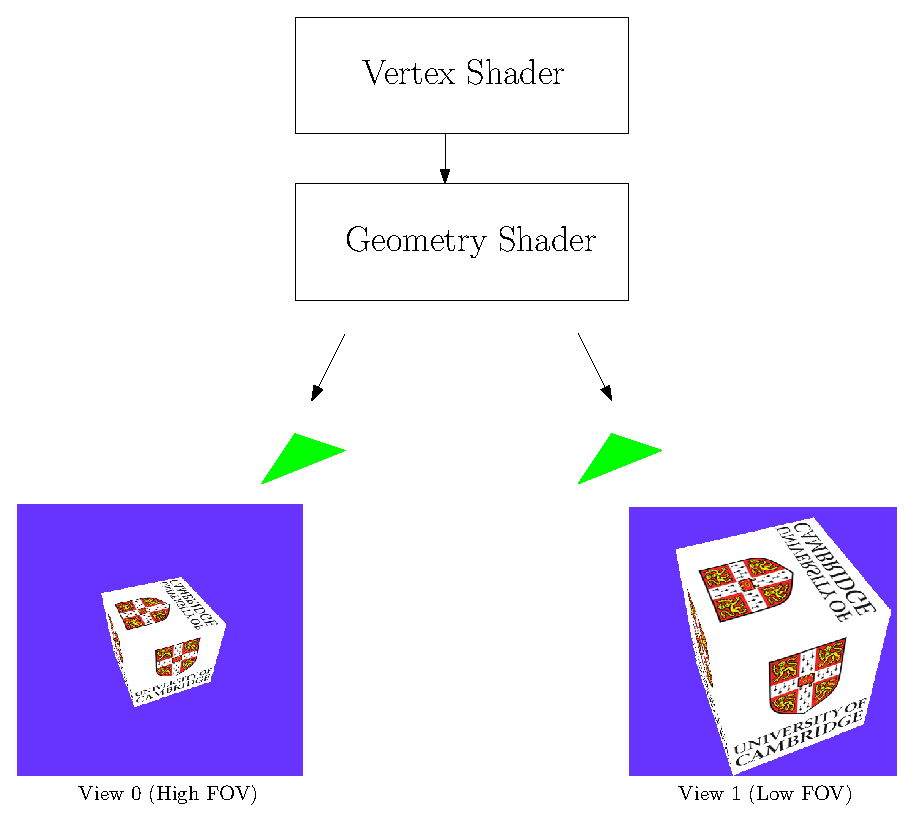
\includegraphics[scale=0.6]{figs/geoshader.eps}}
\caption{Shows the high level process of rendering to two resolutions with one draw call}
\label{epsfig1}
\end{figure}

It's possible to either simultaneously render to separate layers of a layered texture, or simultaneously render to two separate viewports within the same, large texture. I use the latter approach for simplicity. I also assume 4 samples per pixel in this implementation, though it's not difficult to apply this to higher or lower levels of sampling. 

This optimisation requires the OpenGL extension \texttt{ARB\_viewport\_array} though it is near ubiqitous across modern implementations.

First, we must specify our viewports' dimensions:

\begin{blockcode}
float v[] = {0, 0, mWidth, mHeight,
             mWidth, 0, mWidth*2, mHeight};
glViewportArrayv(0, 2, v); //Specify a viewport array, of length 2
\end{blockcode} 

The above initialises a viewport array such that the first viewport occupies the left half of the texture, and the second the right half of the screen. Viewport 0 will have a high field of view rendered to it, while Viewport 1 will have a low field of view, representing the area we will supersample.\\

Next we must enable and compile a geometry shader.

\begin{blockcode}
  layout(triangles) in;
  layout(triangle_strip, max_vertices=6) out;
  ...
  for (i=0; i<2; i++){
    currentProj = i==0 ? proj : projSmall; //select currentProj based on i

    fColour = vColour[0];
    fTexCoord = vTexCoord[0];
    gl_Position = currentProj*view*model*gl_in[0].gl_Position;
    EmitVertex();
    gl_ViewportIndex = i;
  ...
  EndPrimitive();
\end{blockcode}

As required by the geometry shader we first specify the input and output primitive. This same code can be generalised for other primitive types, but triangles are shown here being the general case.
Then we can loop over the viewports, emitting a primitive at each.

Line 5 selects the projection matrix based on the looping variable \texttt{i}. Then, colour, texture and normal information are passed on to the fragment shader for use in lighting and texturing. Finally the position of the vertex is calculated by the standard Model, View, Perspective transformation, Along with the index of the viewport it will be sent to. This snippet is applied to all vertices in the primitive.

The resulting wide framebuffer can then be resolved in the same way given in section AWRAW. We can blit the right half of the screen onto the left half.
Alternatively, you could perform a downsample in the barrel distortion shader, though this alternative wasn't implemented.  

\section{Extension 1: Foveated Rendering}

Foveated rendering refers to the technique of tracking users fovea, so that we can dynamically increase sampling at a fixation point, reducing resolution in the users peripheral. The technique shows promise because only a small field of view around a given fixation point can be percieved in high resolution owing to the number of cones in the fovea.

Given eye-tracking information at the beginning of the frame, ideally a fixation point $(fix_x,fix_y)$ in normalised window coordinates, we can use a very similar technique to the one developed here to perform foveated rendering. The fixation point here is assumed to be in the predistorted window space. 

\subsection{Recalculating projection}

SASDASD defines the perspective projection matrix, given the frustrum parameters $(near, far, top, bottom, left, right)$ of the full field of view, we can calculate a new projection matrix that we can use to render around our fixation point $(fix_x, fix_y)$:

\[
\begin{matrix}
top_{fove}: top \cdot r + fix_y \\
bottom_{fove}: bottom \cdot r + fix_y \\
left_{fove}: left \cdot r + fix_x \\
right_{fove}: right \dot r + fix_x 
\end{matrix}
\]
Where $r$ is a parameter that denotes the ratio of the screen space rendered at high resolution to the space rendered at a lower one. It should be small enough such that the field of view around the fovea is rendered to full resolution, though its value differs based on a large number of factors, including the users proximity to the screen and the size of the screen.

We can then (using the geometry shader approach given in chapter DKAADK) render to two separate viewports. One for a supersampled image around the fovea, and the other for the low resolution peripheral. A method of blending the two images together needs to be made, a blit operation onto the texture passed to the Oculus SDK here will work. 

To reduce artefacts introduced by foveated rendering, extra processing - gaussian blur, increased contrast should be applied to the peripheral image. These weren't implemented, but this extension shows that foveated rendering and subscreen antialiasing can have a close to identical implementation in OpenGL.

\section{Extension 1.5 Non-uniform Texel Density}

Thanks to the barrel distortion, the number of texels per pixel as we move away from the center of the image increases. And because of the nature of graphics APIs, we must render to a higher resolution than needed in the edge of the image, even though this high resolution is only needed in the center, where texel density is relatively uniform and lowest.

If we use the same foveated rendering technique for a fixation point in the centre of the screen, we can shade fewer fragments wilst maintaining at least 1 texel per pixel as a threshold.

We can take this even further and render below the single texel per pixel threshold, exploiting astigmasitm in the lens.

\subsection{Blending the two textures}

A blit operation here might be wasteful, given that the rendertarget is not antialiased, and would require an upscale of the lower resolution texture, wasting GPU memory. So a better method would be to blend the two textures in a post-processing stage. Given that barrel distortion is performed as post-processing, we can blend there. Given access to the fragment shader portion of the barrel distortion shader, every access to the texture provided to the SDK can be modified in the following way:

\begin{blockcode}
insert texture things here.
\end{blockcode}

\section{Limitations}

While some optimisation was allowed for Subscreen Supersampling through the use of the geometry shader, harware support is needed to perform Subscreen Multisampling efficiently. An API extension that allowed for simultaneous drawing to two targets could help to perform Subscreen Multisampling much more efficiently. 

\section{Future Hardware Support}

The disadvantage of the geometry shader approach to multi-resolution shading is the incurred cost of invoking the optional geometry shader stage. I go over this extra cost in section MRAH.
Two extensions to OpenGL have been proposed by Oculus, \texttt{OVR\_MULTIEW}, and \texttt{OVR\_MULTIVIEW2}. These extensions will allow multiple elements of a 2D texture array to be rendered to simultaneously. Allowing us to render both the high resolution central image and lower resolution peripheral in one call, without the need for invoking the geometry shader and without intrusive modifications to the vertex shader. The only implementations of these extensions are in GLES currently - perhaps because of the current lack of a geometry shader stage in GLES.

Regardless, a brief implementation of multi-resolution rendering will be given here.

First we need to set up a layered texture.

\begin{blockcode}
glGenTextures(1, &frameBufferTextureId); //generate a texture
glBindTexture(GL_TEXTURE_2D_ARRAY, frameBufferTextureId);
glTexParameteri(GL_TEXTURE_2D_ARRAY, GL_TEXTURE_MIN_FILTER, GL_LINEAR); //set downsample filter
glTexParameteri(GL_TEXTURE_2D_ARRAY, GL_TEXTURE_MAG_FILTER, GL_LINEAR); //set upscale filter
glTexStorage3D(GL_TEXTURE_2D_ARRAY, 1, GL_RGBA8, mWidth, mHeight, 2); //allocate storage for two textures per eye
\end{blockcode}

Then, a framebuffer must be generated, and the layered texture attached to it.

\begin{blockcode}
glGenFramebuffers(1, &frameBufferObjectId); //Generate a framebuffer
glBindFramebuffer(GL_DRAW_FRAMEBUFFER, frameBufferObjectId); //set framebuffer to be drawn to
glFramebufferTextureMultiviewOVR(GL_DRAW_FRAMEBUFFER, GL_COLOR_ATTACHMENT0, frameBufferTextureId, 0, 0, 2); attach layered texture
\end{blockcode}

Then, we can generate depth buffers for each layer, and attach them to the framebuffer.

\begin{blockcode}
glGenTextures(1, &frameBufferDepthTextureId);
glBindTexture(GL_TEXTURE_2D_ARRAY, frameBufferDepthTextureId);
glTexStorage3D(GL_TEXTURE_2D_ARRAY, 1, GL_DEPTH_COMPONENT24, width, height, 2); //create layered depth texture

glFramebufferTextureMultiviewOVR(GL_DRAW_FRAMEBUFFER, GL_DEPTH_ATTACHMENT, frameBufferDepthTextureId, 0, 0, 2); //attach layered depth texture
\end{blockcode}

Finally, an assertion on framebuffer comepleteness should be made.
\begin{blockcode}
OVR_ASSERT(glCheckFramebufferStatus(GL_DRAW_FRAMEBUFFER) == GL_FRAMEBUFFER_COMPLETE); //assert framebuffer is complete
\end{blockcode}


Then, in a manner similar to selecting a projection matrix based on viewport before, a projection can be selected based on the variable \texttt{gl\_ViewID\_OVR} in the vertex shader like so.

\begin{blockcode}
currentProj = gl_ViewID_OVR == 0 ? proj : projSmall; //select currentProj based on gl_ViewID 
\end{blockcode}

The two textures can be blended in post-processing by the same method given in section ASDSDAK

\chapter{Evaluation}

\section{Subjective Assesment}

A user study was performed to asses the subjective quality across the techniques implemented. The section BLAH describes the experiment, and section NRAH describes its results.

\section{User Study Setup}

Subjects were given 3 different scenes to observe, each with headtracking disabled, and headtracking enabled, across 3 different antialiasing techniques and a control. They were: no antialiasing (control), Fullscreen multisampling (4x),  Subscreen multisampling (4x), Subscreen Supersampling (2x). The latter two being implemented by myself.\\

Test subjects were presented with two images, one after another, and asked to choose the one with better image quality, though the interpretation of better quality was left to the subject. All permutations of image comparison were presented to users, with each experiment taking around 30 minutes. Subjects were also prompted to give verbal feedback describing the reason for their choice.

The three scenes shown were:

\begin{enumerate}
\item A scene of green, untextured blocks, moving in a horizontal circle around the user.\\

\item A scene of a courtyard, including downsampled textures and complex geometry.\\

\item A scene from a balcony, facing a tree with alpha culling to implement leaves.\\

\end{enumerate} 


\section{User study results}

Results varied slightly when headtracking was disabled, possibly owing to the salience of temporal artefacts at polygon edges (flickering) when headtracking was enabled. 

The first scene of moving cubes showed the best 

Subjects Subscreen Supersampling generally performed poorly here, despite offering the best texture filtering of all the techniques. Users complained that the image was noticably, sharp at the centre, and were able to distinguish between the higher quality texture filtering in the centre of the image and the border, and this was pronounced where headtracking was enabled. However Subscreen Supersampling performed the best at the scene of the tree, with spatial artefacts owing to alpha culling being ameliorated only by supersampling.

Fullscreen Multisampling and Subscreen Multisampling were largely indistinguishable, most users had difficulty choosing between them and some made contradictary choices when the image order was reversed. This is might be due to more time fixating on the centre of the screen, but also astigmatism at the edge of the image could help mask artefacts. This seems to be the most promising result from the user study, and backs up the premise on which the project was based.

\section{Objective Assesment}

While the user study performed provides a robust assesment of image quality across different approaches, Computational metrics for objective image quality assesment can be essential. The performance of the system determines how quickly the image resonds to stimulus which can help reduce simulation sickness in the user. Given that implementations of graphics APIs differ dramatically, along with hardware implementations, measuring a framerate directly on a particlar machine cannot be the best indicator of performance as a whole. Though the render time per frame of different approaches are given, it should be understood that performance can vary dramatically across different hardware vendors, graphics APIs and their implementations, and rendering programs. Given this, a range of other information is given to best represent the antialiasing approaches and given some more meaningful insight into their execution. Information such as: triangle count, fragment and vertex shader invocations, API calls, GPU usage, CPU usage, along with some interpretation of this in a platform independent setting.

\section{API calls}

A reduction in the number of API calls we send to the GPU can contribute to better performance of the system. Every API call needs to be send to the GPU and validated, taking hundreds to thousands of instructions.

\begin{center}
\begin{tabular}{l|c|r}
No antialiasing      & 402 \\
Fullscreen Multisampling     & 402 \\
Subscreen Multisampling    &  802  \\
Fullscreen Supersampling      &  402   \\
Subscreen Supersampling    &  403  \\
\end{tabular}
\end{center}

Subscreen Multisampling could not be optimised in the same way as Subscreen Supersampling due to the OpenGL constraint that Complete Framebuffers' Layers must have the same number of samples. Therefore it was neccesary to render the scene twice, explaining why it has twice the number of draw calls.

Subscreen Supersampling has one more draw call than the others because the blending of the two imaage in this implementation was performed in a post-processing step. //VERIFY - IT'S NOT

\section{Fragment shader invocations}

Fragment shader invocations generally increase linearly with the size of image. If our application bottleneck is at the fragment shader stage, we will reap performance benefits by shading less fragments.

\begin{tabular}{l|c|r}
No antialiasing      & 2.3872e+06 \\
Fullscreen Multisampling     & 3.0753e+06 \\
Subscreen Multisampling    &  2.8465e+06  \\
Fullscreen Supersampling      &  7.5106e+06   \\
Subscreen Supersampling    &  3.7955e+06  \\
\end{tabular}

As expected, significantly fewer fragments are shaded in subscreen analogues of fullscreen antialiasing techniques. In this instance Subscreen Multisampling shades 7.6\% fewer fragments, while Subscreen Supersampling shades 49.5\% fewer fragments. 

\subsection{Multisampling}
OpenGL Multisampling will run a fragment shader for every primitive that partially occludes a sample, by taking a sampling rate $r > 1$, which represents the average number of fragment shader invocations per pixel, along with the number of pixels being rendered to $n$, we can calculate at what ratio and screen dimension subscreen multisampling will invoke the fragment shader less than fullscreen multisampling. One invocation of the OpenGL rendering pipeline will shade $\frac{1}{4}n*r + n = (1+\frac{r}{4})n$ fragments in the subcreen case whereas the OpenGL pipeline will shade $n*r$ fragments for fullscreen Multisampling. Using the table in section BRAH, we can calculate a value of $r \approx 1.3$ 

\section{Fragment Shader Timing}

A measurement representing the cumulative time spent processing fragments on the GPU is given below.

\begin{tabular}{l|c|r}
No antialiasing      & 0.30362 \\
Fullscreen Multisampling     & 0.30426 \\
Subscreen Multisampling    &  0.35263  \\
Fullscreen Supersampling      &  0.52043   \\
Subscreen Supersampling    &  0.34764  \\
\end{tabular}

Suprisingly, less time is spent shading fragments in Subscreen Supersampling than in Subscreen Multisampling even though the former invokes the same shader code roughly 1 million times more. This can be attributed to the parralelisation of draw calls in Subscreen Supersampling, whereas Subscreen Multisampling is forced to make double the number of API calls sequentially. It could also be down to the GPU being better able schedule fragment shaders and exploit caches more fully where all invocations happen in one batch.\\

Subscreen Supersampling also outperforms its Fullscreen counterpart, achieving a 33.3\% speedup in the Fragment Shader stage. 

\section{Removal of artefacts}
By capturing views of a scene using different rendering techniques and subtracting them, we can observe artefacts that were present in the scene before and after antialiasing was applied. The image differences below have been thresholded, to make artefacts that have been removed more visible. 

\subsection{Subscreen Supersampling}

\begin{figure}[tbh]
\centerline{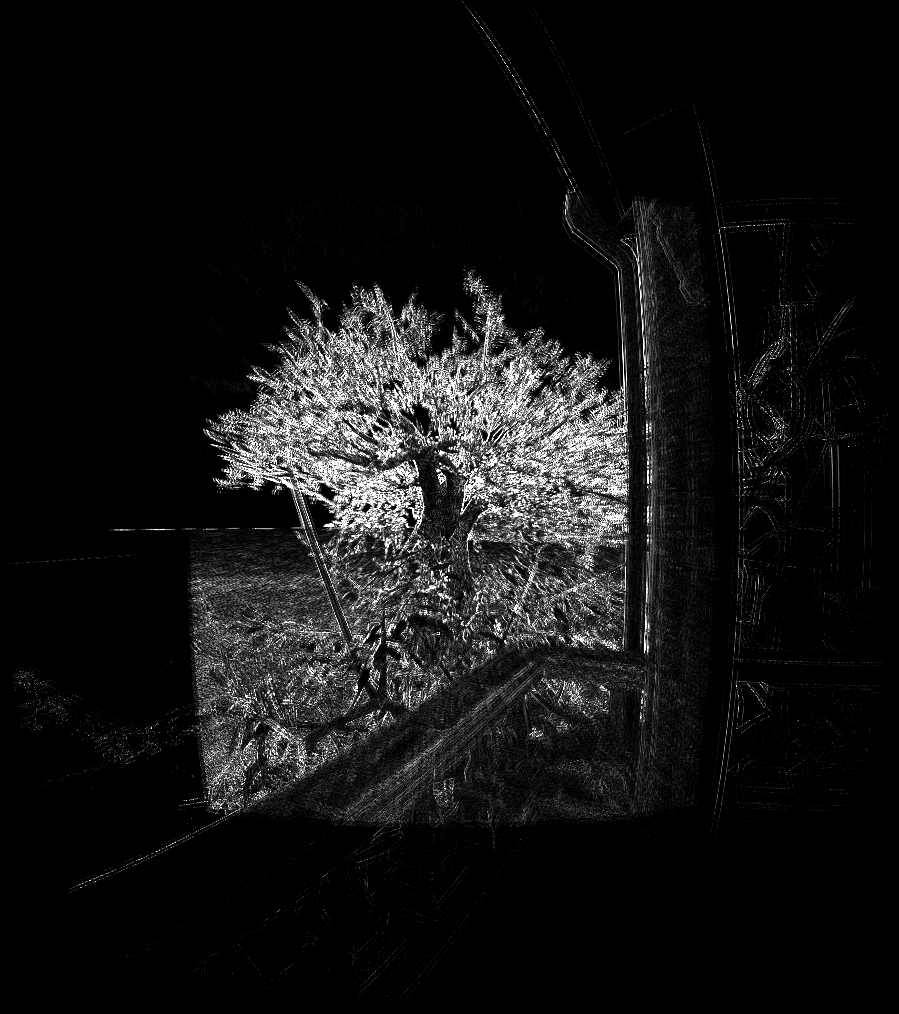
\includegraphics[width=10cm]{figs/difftree.png}}
\caption{Image of the tree scene showing the thresholded difference between Subscreen SSAA and Subscreen MSAA}
\label{ssaatree}
\end{figure}

Using Supersampled Antialiasing, we can see texture filtering has improved. While multisampling only removes artefacts at polygon boundaries. Tree leaves inside of polygons are represented using alpha channel. Supersampling will amerliorate artefacts due to alpha culling, whereas multisampling cannot, hence the large difference between supersampling and multisampling in this scene.

\subsection{Subscreen Multisampling}

\begin{figure}[tbh]
 
\begin{subfigure}{0.5\textwidth}
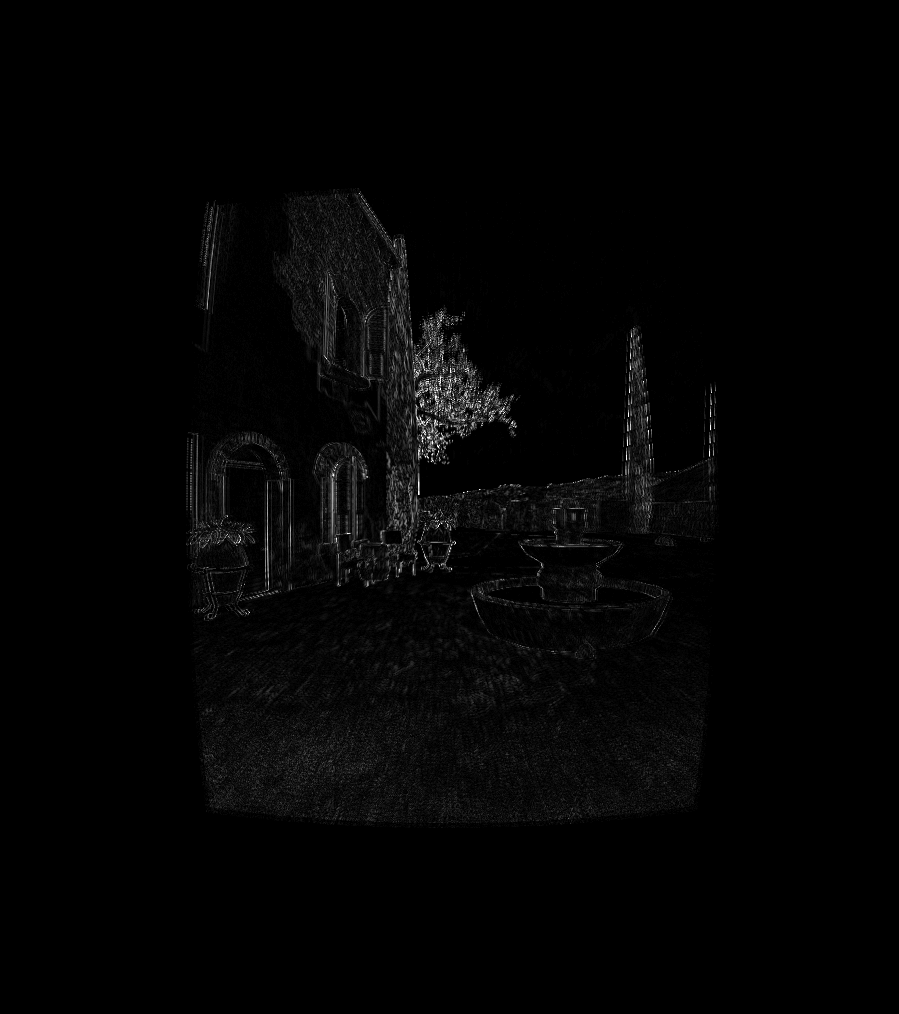
\includegraphics[width=0.9\linewidth, height=5cm]{figs/fullscreenminussubscreenmsaa.png} 
\caption{Caption1}
\label{fig:subim1}
\end{subfigure}
\begin{subfigure}{0.5\textwidth}
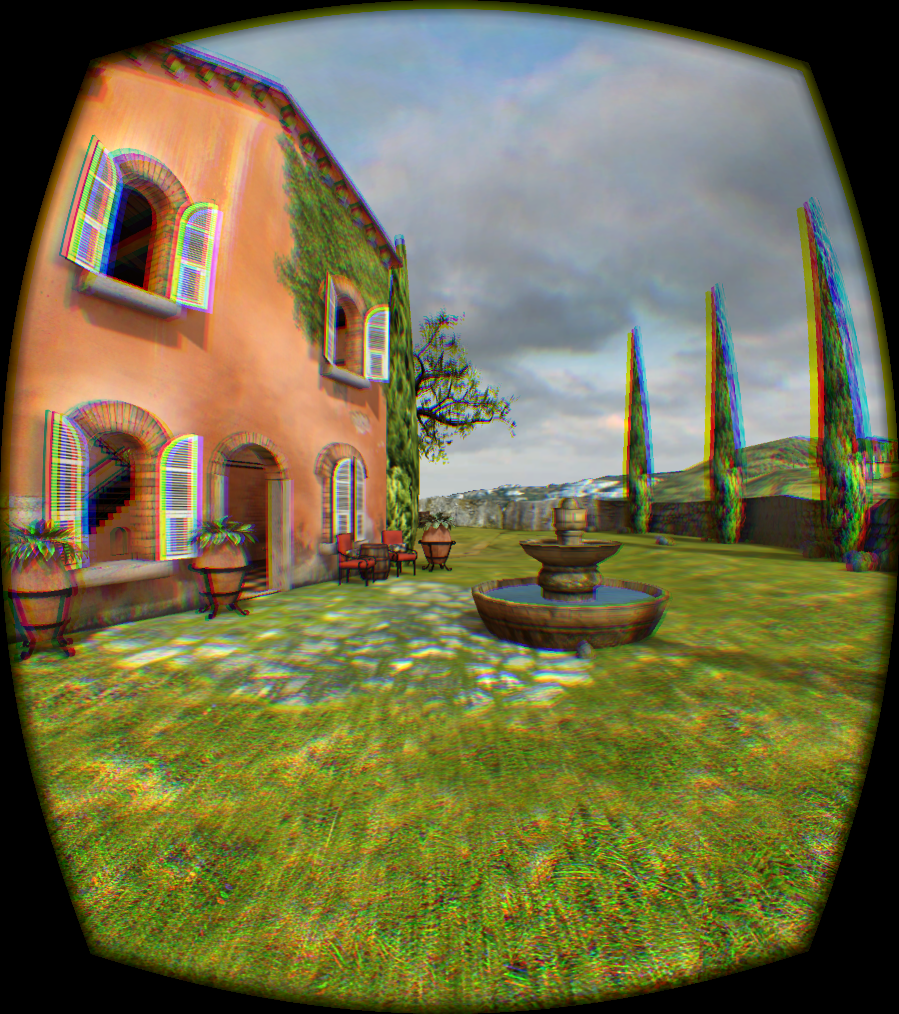
\includegraphics[width=0.9\linewidth, height=5cm]{figs/noantialiasing.png}
\caption{Caption 2}
\label{fig:subim2}
\end{subfigure}
 
\caption{Caption for this figure with two images}
\label{fig:image2}
\end{figure}

Subscreen MSAA works as expected here, artefacts at polygon edges do not differ between fullscreen and subscreen. Interestingly, there is a minute difference in texturing between the two approaches. An explaination for this is a small, subpixel jitter applied to the projection matrix for the central area of the screen, thanks to reduced precision in transforming matrices in section WAT.

\section{Extension 1 Evaluation}



\section{Extension 1.5 Evaluation}

Because of the barrel distortion applied in post-processing Oculus recommends rendering at a resolution \%40 larger than the display permits to achieve an acceptable pixel density in the centre of the image.
A large problem facing the traditional barrel distortion applied in post-processing is a non-uniform pixel density across the image. Futhermore, pixel density is highest at the extremeties, where gaze is less likely to be fixed and lens astigmatism will have the greatest impact. 

\begin{figure}[tbh]
\begin{center}
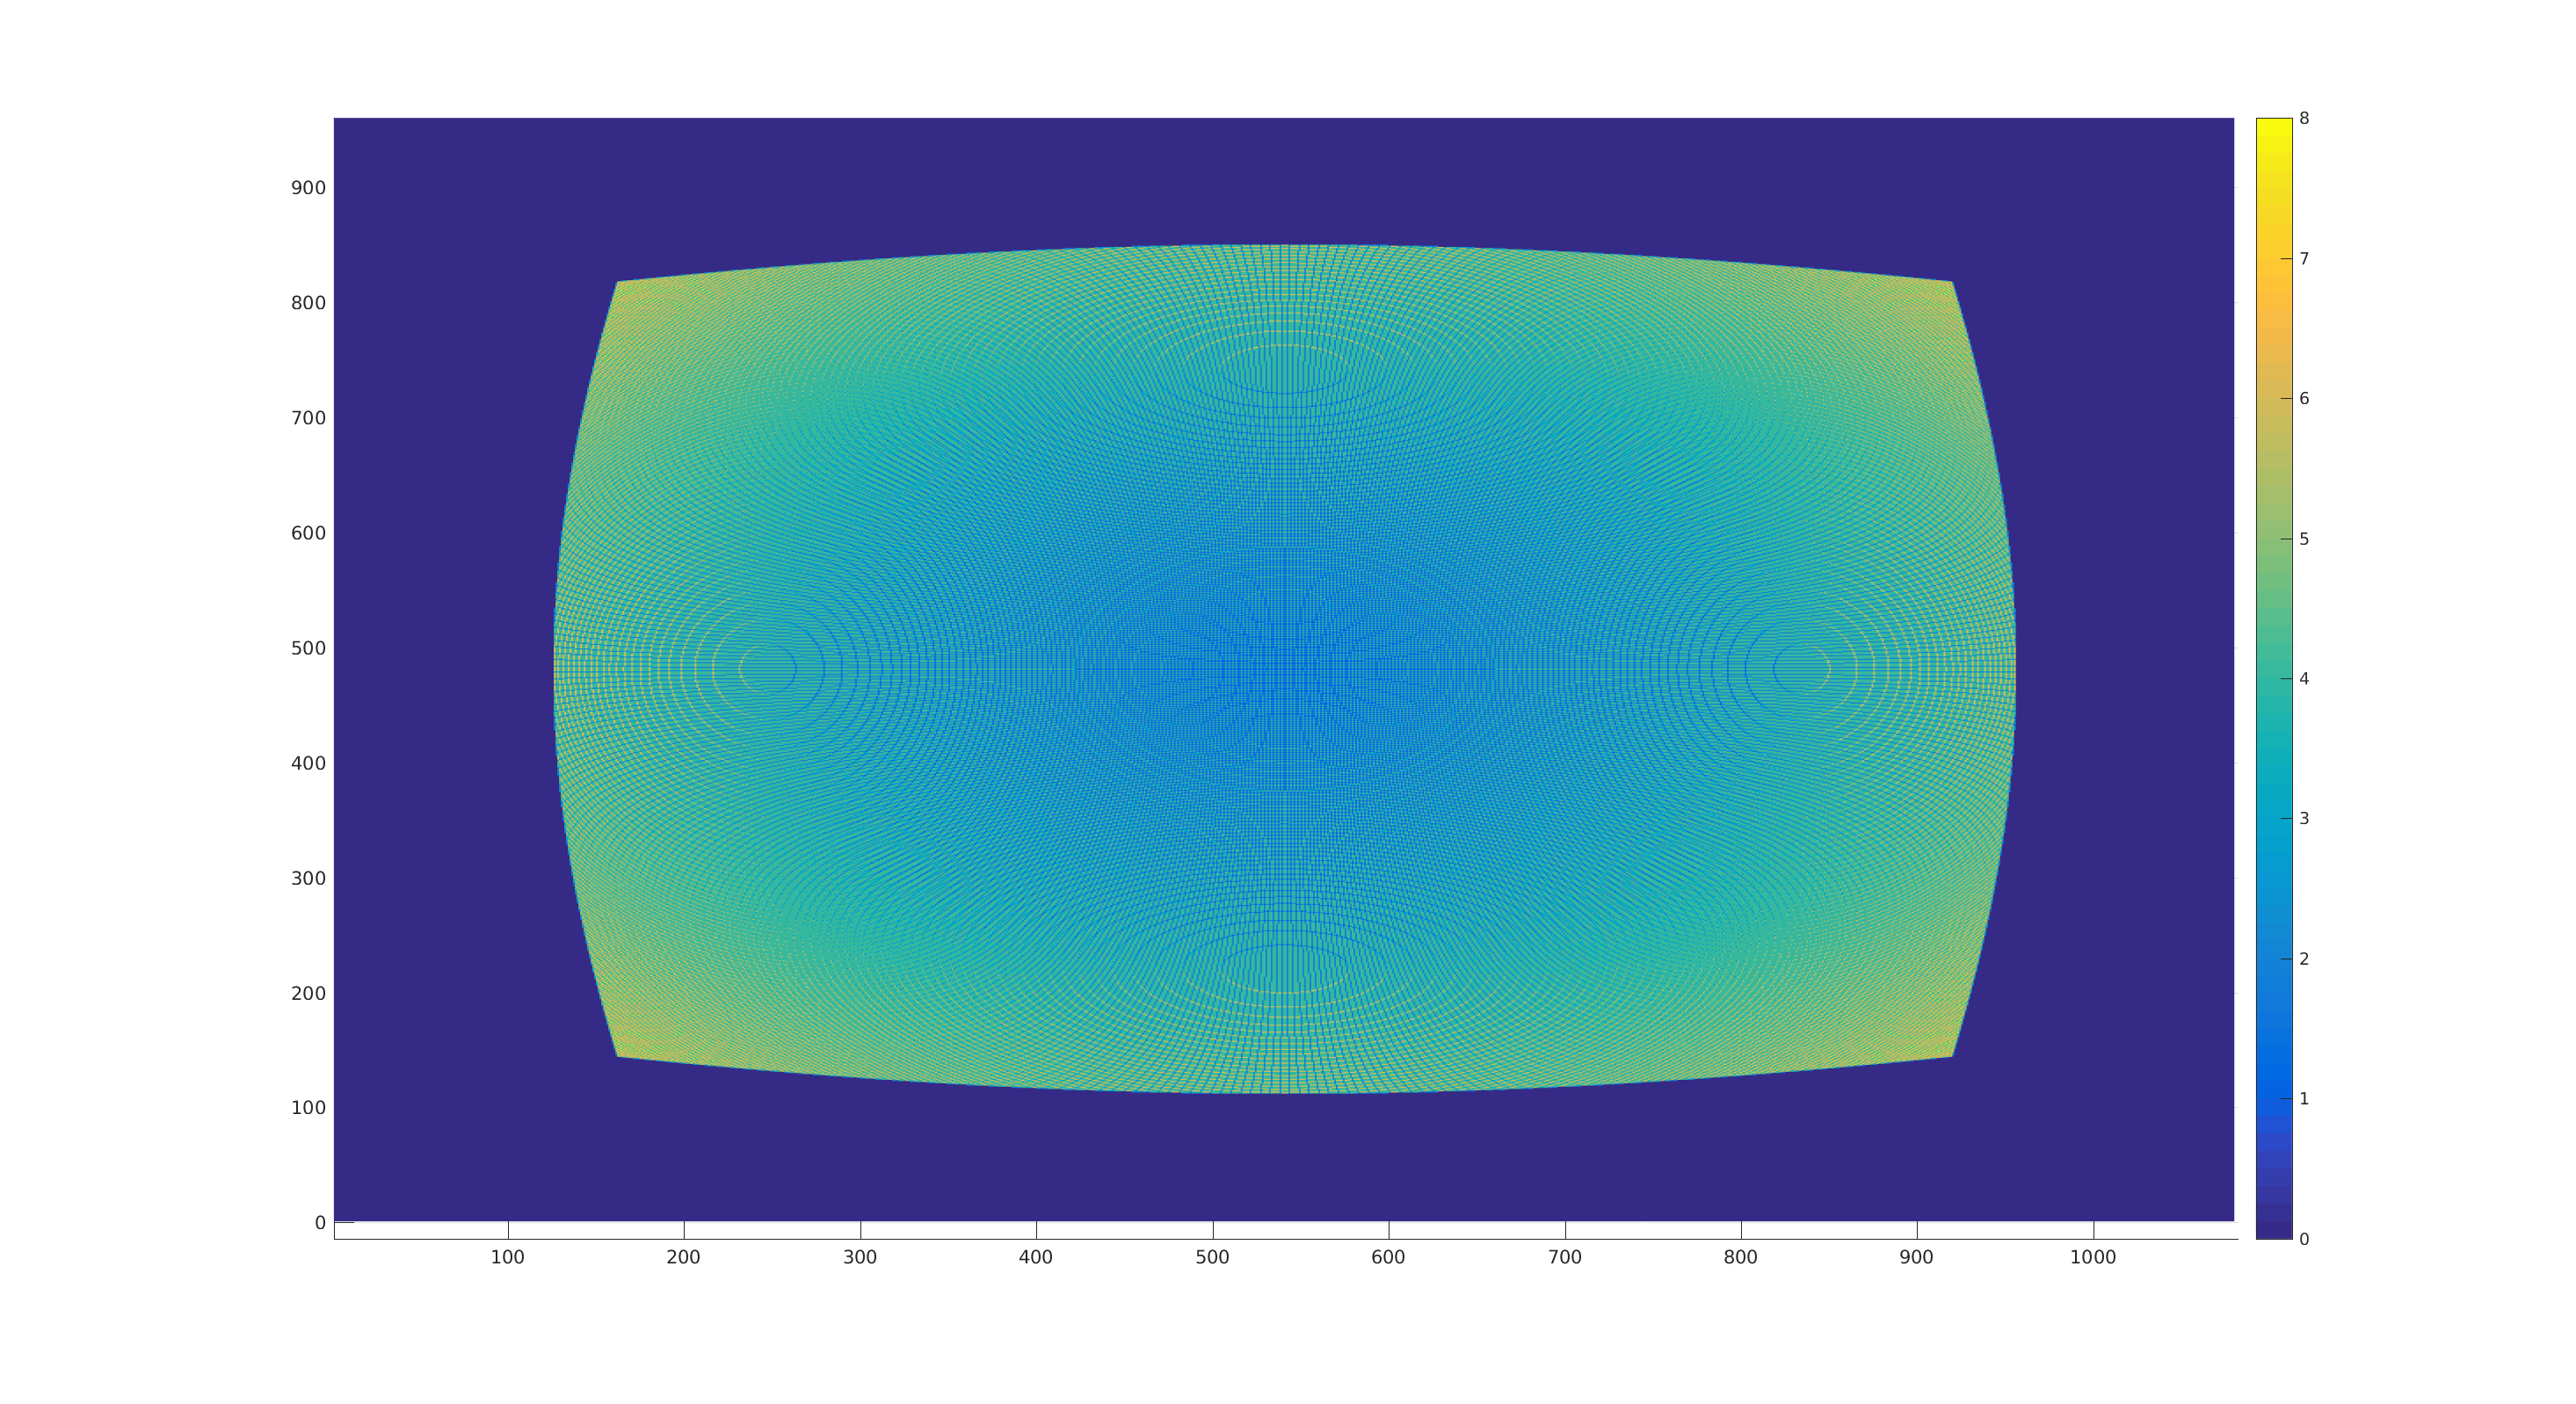
\includegraphics[width=12cm]{figs/oculus_pixel_density.eps}
\caption{Shows the pixel density across an oculus DK2 display post barrel distortion}
\label{epsfig1}
\end{center}
\end{figure}

By only rendering at full resolution in the centre of the image, we improve drastically the pixel density at the center, while decreasing the pixel density in the edges of the image. The number of fragments that we shade is reduced by half, compared to the standard, non-supersampled image size that Oculus recommends. However, twice as many vertices need to be processed. Given that the bottleneck in most consumer applications are in the fragment shader stage, and that we generally need to process significantly more fragments that vertices, we should expect a considerable decrease in the time to present a frame using this method. 

\begin{figure}[tbh]
\begin{center}
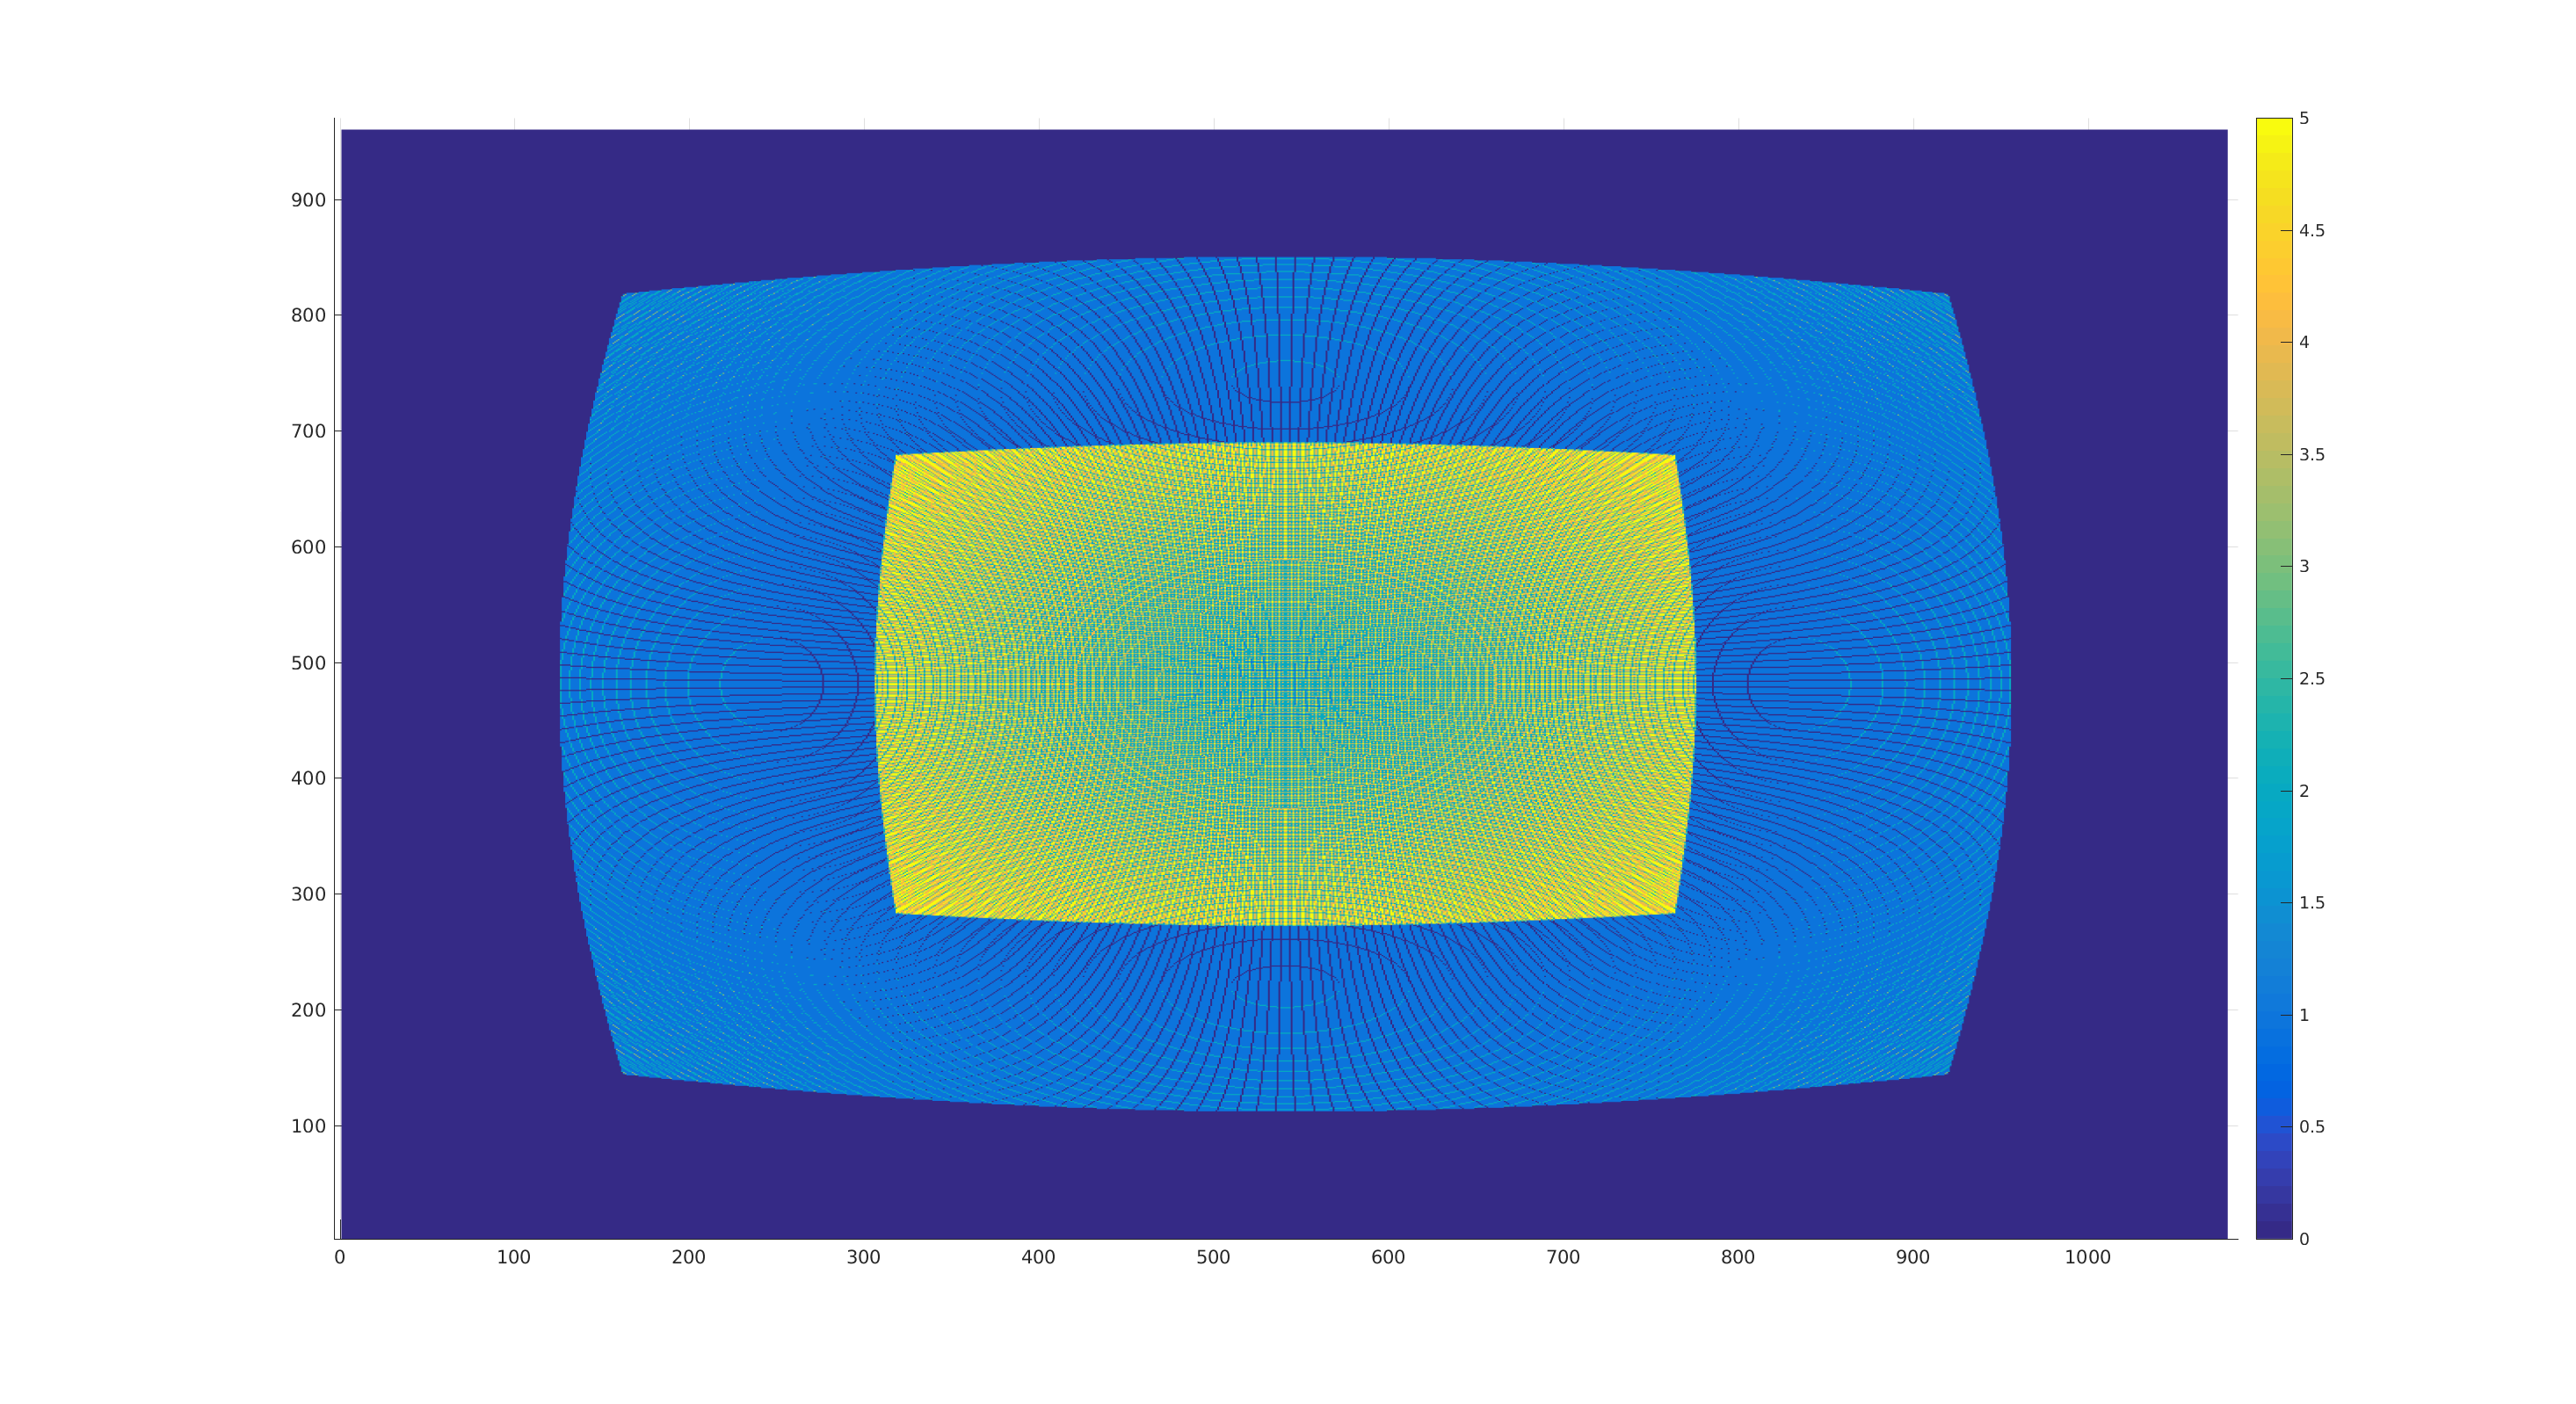
\includegraphics[width=12cm]{figs/oculus_pixel_density_optimisation.eps}
\caption{Shows the pixel density across an oculus DK2 display post barrel distortion}
\label{epsfig1}
\end{center}
\end{figure}




\chapter{Conclusion}



%%%%%%%%%%%%%%%%%%%%%%%%%%%%%%%%%%%%%%%%%%%%%%%%%%%%%%%%%%%%%%%%%%%%%
% the bibliography
\addcontentsline{toc}{chapter}{Bibliography}
\bibliography{refs}

%%%%%%%%%%%%%%%%%%%%%%%%%%%%%%%%%%%%%%%%%%%%%%%%%%%%%%%%%%%%%%%%%%%%%
% the appendices
\appendix

\chapter{Latex source}

\section{diss.tex}
{\scriptsize\verbatiminput{diss.tex}}

\section{proposal.tex}
{\scriptsize\verbatiminput{proposal.tex}}

\chapter{Makefile}

\section{makefile}\label{makefile}
{\scriptsize\verbatiminput{makefile.txt}}

\section{refs.bib}
{\scriptsize\verbatiminput{refs.bib}}


\chapter{Project Proposal}

% Note: this file can be compiled on its own, but is also included by
% diss.tex (using the docmute.sty package to ignore the preamble)
\documentclass[12pt,a4paper,twoside]{article}
\usepackage[pdfborder={0 0 0}]{hyperref}
\usepackage[margin=25mm]{geometry}
\usepackage{graphicx}
\usepackage{parskip}
\begin{document}

\begin{center}
\Large
Computer Science Tripos -- Part II -- Project Proposal\\[4mm]
\LARGE
Smart Anti-Aliasing for Virtual Reality \\[4mm]

\large
G.~Ash, Fitzwilliam College

12 October 2016
\end{center}

\vspace{5mm}

\textbf{Project Supervisor:} Dr R.~Mantiuk

\textbf{Director of Studies:} Dr R.~Harle

\textbf{Project Overseers:} Prof R.~Anderson  \& Prof J.~Bacon

% Main document

\section*{Introduction}

A problem with modern Virtual Reality headsets is that they use low resolution displays to cover a huge Field of View.
Graphical artefacts, such as moir\'e patterns and pixellated edges (jaggies), are pronounced on these displays.
A good technique to ameliorate these artefacts if super-sampling, but super-sampling is often too expensive in VR
devices where low latency is a requirement - to avoid simulation sickness. 

Unfortunately, modern consumer headsets suffer from astigmatism because of a single lens between the viewer and the display. We can't remove these distortions without (another) anastigmatic lens, however we do currently give equal preference to image quality across the whole of the display even when the edges of the image become distorted.

\begin{figure}[tbh]
\centerline{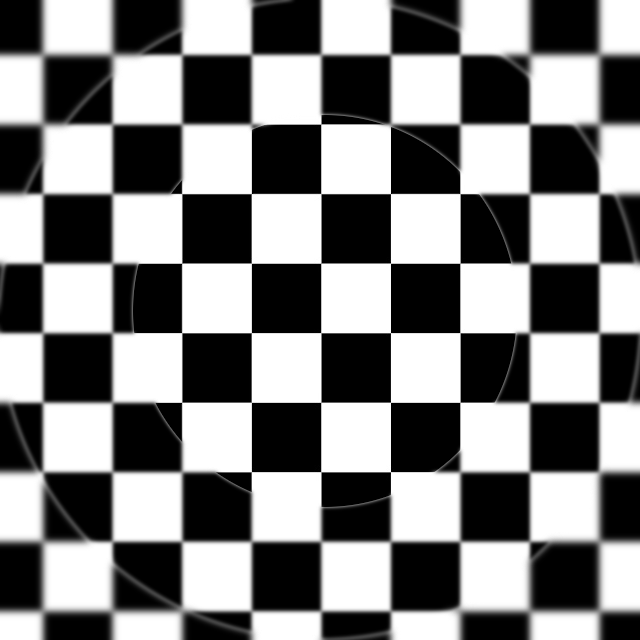
\includegraphics[width=0.3\linewidth]{figs/blur.png}}
\caption{The center of the perceived image is sharp, while the edges get progressively blurrier}
\label{blurfig}
\end{figure}

We could exploit astigmatism in single lens VR headsets by sampling more in the sharp center of the image,
and sampling less as we move towards the blurrier edges (Figure \ref{blurfig}). This project aims to extend an existing open source system to include this optimisation, and to measure the impact on both the performance of the system, and on the image quality to the user.

\section*{Starting point}

Novel anti-aliasing techniques, such as subpixel-reconstruction and temporal antialiasing, are still actively being developed. I intend to build on Intel's research[1] into a hybrid raytracing/rasterizing VR renderer by creating an entirely rasterized solution that retains image quality while allowing for GPU hardware acceleration.

Free and extensible renderers exist for VR headsets, such as Unity. However I will be extending the existing open-source OSVR-RenderManager, which will allow me to easily create separate reusable demos to show off certain graphical artefacts, and, if neccesary, to modify the entire rendering pipeline.
OSVR is compatible with all modern VR headsets, and supports all modern graphics APIs (OpenGL, Vulkan, Direct3D).

I have good experience in C/C++ through small projects and the IB C/C++ course. I'm familiar with the graphics pipeline and have experience in WebGL, with some experience writing vertex and fragment shaders in OpenGL. I will need to refresh my knowledge of shader programming, and will need to take some time learning most of the OpenGL API.

\section*{Resources required}

For this project I shall be using my own quad-core machine with a VR capable GPU. I will also be using an Occulus Rift Development Kit 2 [3](lent to me by the Hackers at Cambridge group) for testing and user studies. Source backups will be made both to a private Github repository and MCS daily.
I will use an MCS machine as a failsafe incase my machine should break.

\section*{Work to be done}

The project breaks down into the following sub-projects:

\begin{enumerate}

\item \textbf{Setup} Fork the existing Open Source Virtual Reality-RenderManager repository. Create a daily cronjob to backup this to github and MCS. Research my chosen renderer's pipeline.

\item \textbf {Core development} Develop/modify a simple super-sampling algorithm. Extend the algorithm to allow for areas of the screen to be ignored. Further extend to seamlessly composite draws that we sample differently.

\item \textbf {Demo creation} Create a couple of OpenGL demos that highlight both moire patterns and pixellated edges, for use in visual quality experiment.

\item \textbf {Optimisation} Make use of a GPU profiler to determine any redundancy or inefficiency. Refactor the algorithm to make it easily configurable.

\item \textbf {Evaluation} Make use of benchmarking/profiling software to evaluate the algorithm with regards to performance. Perform visual quality experiment to evaluate the impact of the algorithm on image quality to the user, recruit college members across fields to participate. Compare my approach against no anti-aliasing, and fullscreen anti-aliasing.

\end{enumerate}

\section*{Success citeria}

The project will be a success if I manage to do the following:
\begin{enumerate}

\item Improve the performance of the open source renderer with anti-aliasing enabled

\item Provide an alternative anti-aliasing technique that suffers only negligible loss in image quality to the end user.

\item Evaluate both full screen antialiasing, my selective antialiasing approach, and no antialiasing from a user perspective by constructing demos that show off artefacts masked by antialiasing.

\end{enumerate}

\section*{Possible extensions}

If I achieve my main result early I shall try the following
alternative experiment or method of evaluation:

\begin{enumerate}

\item Research using a heuristic to determine salient objects or regions in the scene, and extend my algorithm to more closely resemble a foveated rendering[2] technique.

\item Further reduce the requirement to super-sample by determining which objects/samples can be shared between each eye.

\end{enumerate}





\section*{Timetable}

Planned starting date is 16/10/2011.

\begin{enumerate}

\item \textbf{Michaelmas weeks 2--4} Start project Setup, Begin refreshing knowledge on OpenGL. Research the rendering pipeline of my chosen renderer. Formulate an implementation strategy.

\item \textbf{Michaelmas weeks 5--6} Complete project setup. Test writing custom code in the renderer, start implementation of selective antialiasing algorithm

\item \textbf{Michaelmas weeks 7--8} Continue development of algorithm. Start on demo creation

\item \textbf{Michaelmas vacation} Finish development of algorithm and demos.

\item \textbf{Lent weeks 0--2} Write progress report. Generate corpus of
  test examples. Begin optimisation.

\item \textbf{Lent weeks 3--5} Finish optimisation, begin evaluation of image quality on users.  

\item \textbf{Lent weeks 6--8} Finish user studies, start performance analysis. Write up User studies in disseration.

\item \textbf{Easter vacation:} Begin on extensions, flesh out dissertation, complete evaluation. 

\item \textbf{Easter term 0--2:}  Complete dissertation, proof read. Submit to DoS and supervisor for comments. 

\item \textbf{Easter term 3:} Further proof reading/refactoring and submit dissertation.

\end{enumerate}

\section*{References}

\begin{enumerate}

\item Using Astigmatism in Wide Angle HMDs to Improve Rendering D. Pohl, T. Bolkart, S. Nickels, O. Grau, 2015.
\item Foveated 3d graphics. B. Guenter, M. Finch, S. Drucker, D. Tan, and J. Snyder. ACM SIGGRAPH Asia, 2012.
\item Oculus VR. Oculus Rift, 2014. http://www.oculus.com/

\end{enumerate}

\end{document}


\end{document}
